\documentclass{standalone}
\usepackage{tikz}
\usetikzlibrary{patterns, positioning}


\begin{document}
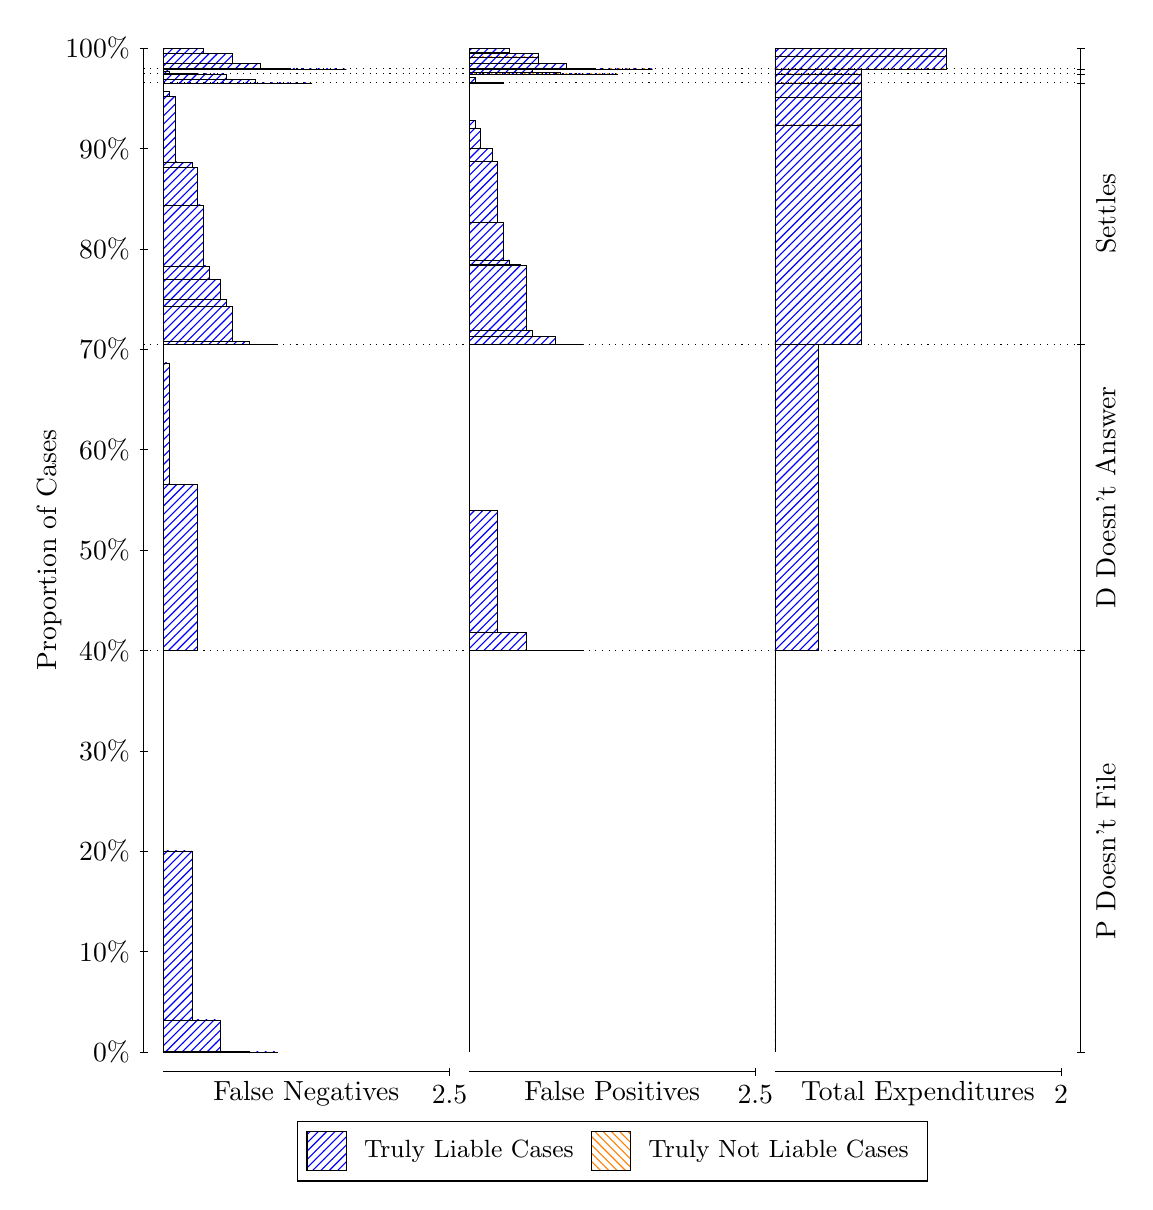
\begin{tikzpicture}
\draw[black, very thin] (1.5,1.75) -- (1.5,14.5);
\node[rotate=90, text=black, anchor=center] at (0.3, 8.125) {Proportion of Cases};
\draw[black, very thin] (1.45,1.75) -- (1.55,1.75);
\node[text=black, anchor=east] at (1.45, 1.75) {0\%};
\draw[black, very thin] (1.45,3.025) -- (1.55,3.025);
\node[text=black, anchor=east] at (1.45, 3.025) {10\%};
\draw[black, very thin] (1.45,4.3) -- (1.55,4.3);
\node[text=black, anchor=east] at (1.45, 4.3) {20\%};
\draw[black, very thin] (1.45,5.575) -- (1.55,5.575);
\node[text=black, anchor=east] at (1.45, 5.575) {30\%};
\draw[black, very thin] (1.45,6.85) -- (1.55,6.85);
\node[text=black, anchor=east] at (1.45, 6.85) {40\%};
\draw[black, very thin] (1.45,8.125) -- (1.55,8.125);
\node[text=black, anchor=east] at (1.45, 8.125) {50\%};
\draw[black, very thin] (1.45,9.4) -- (1.55,9.4);
\node[text=black, anchor=east] at (1.45, 9.4) {60\%};
\draw[black, very thin] (1.45,10.675) -- (1.55,10.675);
\node[text=black, anchor=east] at (1.45, 10.675) {70\%};
\draw[black, very thin] (1.45,11.95) -- (1.55,11.95);
\node[text=black, anchor=east] at (1.45, 11.95) {80\%};
\draw[black, very thin] (1.45,13.225) -- (1.55,13.225);
\node[text=black, anchor=east] at (1.45, 13.225) {90\%};
\draw[black, very thin] (1.45,14.5) -- (1.55,14.5);
\node[text=black, anchor=east] at (1.45, 14.5) {100\%};

\draw[black, very thin] (13.4,1.75) -- (13.4,14.5);
\draw[black, very thin] (13.35,1.75) -- (13.45,1.75);
\node[anchor=west] at (13.35, 1.75) {};
\draw[black, very thin] (13.35,6.8489) -- (13.45,6.8489);
\node[anchor=west] at (13.35, 6.8489) {};
\draw[black, very thin] (13.35,10.735) -- (13.45,10.735);
\node[anchor=west] at (13.35, 10.735) {};
\draw[black, very thin] (13.35,14.058) -- (13.45,14.058);
\node[anchor=west] at (13.35, 14.058) {};
\draw[black, very thin] (13.35,14.172) -- (13.45,14.172);
\node[anchor=west] at (13.35, 14.172) {};
\draw[black, very thin] (13.35,14.235) -- (13.45,14.235);
\node[anchor=west] at (13.35, 14.235) {};
\draw[black, very thin] (13.35,14.5) -- (13.45,14.5);
\node[anchor=west] at (13.35, 14.5) {};

\draw[black, very thin, pattern color=blue, pattern=north east lines] (1.75,1.75) rectangle (3.2033,1.75);
\draw[black, very thin, pattern color=blue, pattern=north east lines] (1.75,1.75) rectangle (2.84,1.7534);
\draw[black, very thin, pattern color=blue, pattern=north east lines] (1.75,1.7534) rectangle (2.4767,2.158);
\draw[black, very thin, pattern color=blue, pattern=north east lines] (1.75,2.158) rectangle (2.1133,4.3029);
\draw[black, very thin, pattern color=orange, pattern=north west lines] (1.75,4.3029) rectangle (1.75,4.3029);
\draw[black, very thin, pattern color=blue, pattern=north east lines] (1.75,4.3029) rectangle (1.75,6.8489);
\draw[black, very thin, pattern color=blue, pattern=north east lines] (1.75,6.8489) rectangle (2.186,8.9591);
\draw[black, very thin, pattern color=blue, pattern=north east lines] (1.75,8.9591) rectangle (1.8227,10.5);
\draw[black, very thin, pattern color=orange, pattern=north west lines] (1.75,10.5) rectangle (1.75,10.5);
\draw[black, very thin, pattern color=blue, pattern=north east lines] (1.75,10.5) rectangle (1.75,10.735);
\draw[black, very thin, pattern color=blue, pattern=north east lines] (1.75,10.735) rectangle (3.2033,10.735);
\draw[black, very thin, pattern color=blue, pattern=north east lines] (1.75,10.735) rectangle (3.058,10.735);
\draw[black, very thin, pattern color=blue, pattern=north east lines] (1.75,10.735) rectangle (2.9127,10.735);
\draw[black, very thin, pattern color=blue, pattern=north east lines] (1.75,10.735) rectangle (2.84,10.77);
\draw[black, very thin, pattern color=blue, pattern=north east lines] (1.75,10.77) rectangle (2.6947,10.779);
\draw[black, very thin, pattern color=blue, pattern=north east lines] (1.75,10.779) rectangle (2.622,11.216);
\draw[black, very thin, pattern color=blue, pattern=north east lines] (1.75,11.216) rectangle (2.5493,11.312);
\draw[black, very thin, pattern color=blue, pattern=north east lines] (1.75,11.312) rectangle (2.4767,11.563);
\draw[black, very thin, pattern color=blue, pattern=north east lines] (1.75,11.563) rectangle (2.3313,11.733);
\draw[black, very thin, pattern color=blue, pattern=north east lines] (1.75,11.733) rectangle (2.2587,12.507);
\draw[black, very thin, pattern color=blue, pattern=north east lines] (1.75,12.507) rectangle (2.186,12.983);
\draw[black, very thin, pattern color=blue, pattern=north east lines] (1.75,12.983) rectangle (2.1133,13.044);
\draw[black, very thin, pattern color=blue, pattern=north east lines] (1.75,13.044) rectangle (1.968,13.053);
\draw[black, very thin, pattern color=blue, pattern=north east lines] (1.75,13.053) rectangle (1.8953,13.882);
\draw[black, very thin, pattern color=blue, pattern=north east lines] (1.75,13.882) rectangle (1.8227,13.952);
\draw[black, very thin, pattern color=orange, pattern=north west lines] (1.75,13.952) rectangle (1.75,13.952);
\draw[black, very thin, pattern color=blue, pattern=north east lines] (1.75,13.952) rectangle (1.75,14.058);
\draw[black, very thin, pattern color=blue, pattern=north east lines] (1.75,14.058) rectangle (3.6393,14.058);
\draw[black, very thin, pattern color=blue, pattern=north east lines] (1.75,14.058) rectangle (3.276,14.058);
\draw[black, very thin, pattern color=blue, pattern=north east lines] (1.75,14.058) rectangle (2.9127,14.101);
\draw[black, very thin, pattern color=blue, pattern=north east lines] (1.75,14.101) rectangle (2.5493,14.171);
\draw[black, very thin, pattern color=blue, pattern=north east lines] (1.75,14.171) rectangle (2.186,14.172);
\draw[black, very thin, pattern color=orange, pattern=north west lines] (1.75,14.172) rectangle (1.75,14.172);
\draw[black, very thin, pattern color=blue, pattern=north east lines] (1.75,14.172) rectangle (2.186,14.173);
\draw[black, very thin, pattern color=blue, pattern=north east lines] (1.75,14.173) rectangle (1.8227,14.211);
\draw[black, very thin, pattern color=orange, pattern=north west lines] (1.75,14.211) rectangle (1.75,14.211);
\draw[black, very thin, pattern color=blue, pattern=north east lines] (1.75,14.211) rectangle (1.75,14.235);
\draw[black, very thin, pattern color=blue, pattern=north east lines] (1.75,14.235) rectangle (4.0753,14.235);
\draw[black, very thin, pattern color=blue, pattern=north east lines] (1.75,14.235) rectangle (3.712,14.235);
\draw[black, very thin, pattern color=blue, pattern=north east lines] (1.75,14.235) rectangle (3.3487,14.239);
\draw[black, very thin, pattern color=blue, pattern=north east lines] (1.75,14.239) rectangle (2.9853,14.3);
\draw[black, very thin, pattern color=blue, pattern=north east lines] (1.75,14.3) rectangle (2.622,14.434);
\draw[black, very thin, pattern color=blue, pattern=north east lines] (1.75,14.434) rectangle (2.2587,14.495);
\draw[black, very thin, pattern color=blue, pattern=north east lines] (1.75,14.495) rectangle (1.8953,14.5);
\draw[black, very thin, pattern color=orange, pattern=north west lines] (1.75,14.5) rectangle (1.75,14.5);
\draw[black, very thin, pattern color=blue, pattern=north east lines] (1.75,14.5) rectangle (1.75,14.5);
\draw[black, very thin, pattern color=orange, pattern=north west lines] (5.6333,1.75) rectangle (5.6333,1.75);
\draw[black, very thin, pattern color=blue, pattern=north east lines] (5.6333,1.75) rectangle (5.6333,6.8489);
\draw[black, very thin, pattern color=orange, pattern=north west lines] (5.6333,6.8489) rectangle (7.0867,6.8489);
\draw[black, very thin, pattern color=blue, pattern=north east lines] (5.6333,6.8489) rectangle (7.0867,6.8489);
\draw[black, very thin, pattern color=blue, pattern=north east lines] (5.6333,6.8489) rectangle (6.7233,6.8492);
\draw[black, very thin, pattern color=blue, pattern=north east lines] (5.6333,6.8492) rectangle (6.36,7.0834);
\draw[black, very thin, pattern color=blue, pattern=north east lines] (5.6333,7.0834) rectangle (5.9967,8.6243);
\draw[black, very thin, pattern color=blue, pattern=north east lines] (5.6333,8.6243) rectangle (5.6333,10.735);
\draw[black, very thin, pattern color=orange, pattern=north west lines] (5.6333,10.735) rectangle (7.0867,10.735);
\draw[black, very thin, pattern color=blue, pattern=north east lines] (5.6333,10.735) rectangle (7.0867,10.735);
\draw[black, very thin, pattern color=orange, pattern=north west lines] (5.6333,10.735) rectangle (6.796,10.735);
\draw[black, very thin, pattern color=blue, pattern=north east lines] (5.6333,10.735) rectangle (6.796,10.735);
\draw[black, very thin, pattern color=blue, pattern=north east lines] (5.6333,10.735) rectangle (6.7233,10.841);
\draw[black, very thin, pattern color=orange, pattern=north west lines] (5.6333,10.841) rectangle (6.6507,10.841);
\draw[black, very thin, pattern color=blue, pattern=north east lines] (5.6333,10.841) rectangle (6.6507,10.841);
\draw[black, very thin, pattern color=orange, pattern=north west lines] (5.6333,10.841) rectangle (6.5053,10.841);
\draw[black, very thin, pattern color=blue, pattern=north east lines] (5.6333,10.841) rectangle (6.5053,10.841);
\draw[black, very thin, pattern color=blue, pattern=north east lines] (5.6333,10.841) rectangle (6.4327,10.911);
\draw[black, very thin, pattern color=blue, pattern=north east lines] (5.6333,10.911) rectangle (6.36,11.74);
\draw[black, very thin, pattern color=blue, pattern=north east lines] (5.6333,11.74) rectangle (6.2873,11.749);
\draw[black, very thin, pattern color=blue, pattern=north east lines] (5.6333,11.749) rectangle (6.142,11.81);
\draw[black, very thin, pattern color=blue, pattern=north east lines] (5.6333,11.81) rectangle (6.0693,12.286);
\draw[black, very thin, pattern color=blue, pattern=north east lines] (5.6333,12.286) rectangle (5.9967,13.06);
\draw[black, very thin, pattern color=blue, pattern=north east lines] (5.6333,13.06) rectangle (5.924,13.23);
\draw[black, very thin, pattern color=blue, pattern=north east lines] (5.6333,13.23) rectangle (5.7787,13.481);
\draw[black, very thin, pattern color=blue, pattern=north east lines] (5.6333,13.481) rectangle (5.706,13.577);
\draw[black, very thin, pattern color=blue, pattern=north east lines] (5.6333,13.577) rectangle (5.6333,14.058);
\draw[black, very thin, pattern color=orange, pattern=north west lines] (5.6333,14.058) rectangle (6.0693,14.058);
\draw[black, very thin, pattern color=blue, pattern=north east lines] (5.6333,14.058) rectangle (6.0693,14.06);
\draw[black, very thin, pattern color=blue, pattern=north east lines] (5.6333,14.06) rectangle (5.706,14.129);
\draw[black, very thin, pattern color=blue, pattern=north east lines] (5.6333,14.129) rectangle (5.6333,14.172);
\draw[black, very thin, pattern color=orange, pattern=north west lines] (5.6333,14.172) rectangle (7.5227,14.172);
\draw[black, very thin, pattern color=blue, pattern=north east lines] (5.6333,14.172) rectangle (7.5227,14.172);
\draw[black, very thin, pattern color=blue, pattern=north east lines] (5.6333,14.172) rectangle (7.1593,14.172);
\draw[black, very thin, pattern color=blue, pattern=north east lines] (5.6333,14.172) rectangle (6.796,14.195);
\draw[black, very thin, pattern color=blue, pattern=north east lines] (5.6333,14.195) rectangle (6.4327,14.234);
\draw[black, very thin, pattern color=blue, pattern=north east lines] (5.6333,14.234) rectangle (6.0693,14.235);
\draw[black, very thin, pattern color=orange, pattern=north west lines] (5.6333,14.235) rectangle (7.9587,14.235);
\draw[black, very thin, pattern color=blue, pattern=north east lines] (5.6333,14.235) rectangle (7.9587,14.235);
\draw[black, very thin, pattern color=orange, pattern=north west lines] (5.6333,14.235) rectangle (7.5953,14.235);
\draw[black, very thin, pattern color=blue, pattern=north east lines] (5.6333,14.235) rectangle (7.5953,14.235);
\draw[black, very thin, pattern color=orange, pattern=north west lines] (5.6333,14.235) rectangle (7.232,14.235);
\draw[black, very thin, pattern color=blue, pattern=north east lines] (5.6333,14.235) rectangle (7.232,14.239);
\draw[black, very thin, pattern color=blue, pattern=north east lines] (5.6333,14.239) rectangle (6.8687,14.3);
\draw[black, very thin, pattern color=orange, pattern=north west lines] (5.6333,14.3) rectangle (6.8687,14.3);
\draw[black, very thin, pattern color=blue, pattern=north east lines] (5.6333,14.3) rectangle (6.8687,14.301);
\draw[black, very thin, pattern color=blue, pattern=north east lines] (5.6333,14.301) rectangle (6.5053,14.388);
\draw[black, very thin, pattern color=orange, pattern=north west lines] (5.6333,14.388) rectangle (6.5053,14.388);
\draw[black, very thin, pattern color=blue, pattern=north east lines] (5.6333,14.388) rectangle (6.5053,14.435);
\draw[black, very thin, pattern color=blue, pattern=north east lines] (5.6333,14.435) rectangle (6.142,14.448);
\draw[black, very thin, pattern color=blue, pattern=north east lines] (5.6333,14.448) rectangle (6.142,14.496);
\draw[black, very thin, pattern color=blue, pattern=north east lines] (5.6333,14.496) rectangle (5.7787,14.496);
\draw[black, very thin, pattern color=blue, pattern=north east lines] (5.6333,14.496) rectangle (5.7787,14.5);
\draw[black, very thin, pattern color=blue, pattern=north east lines] (5.6333,14.5) rectangle (5.6333,14.5);
\draw[black, very thin, pattern color=orange, pattern=north west lines] (9.5167,1.75) rectangle (9.5167,1.75);
\draw[black, very thin, pattern color=blue, pattern=north east lines] (9.5167,1.75) rectangle (9.5167,6.8489);
\draw[black, very thin, pattern color=orange, pattern=north west lines] (9.5167,6.8489) rectangle (10.062,6.8489);
\draw[black, very thin, pattern color=blue, pattern=north east lines] (9.5167,6.8489) rectangle (10.062,10.735);
\draw[black, very thin, pattern color=orange, pattern=north west lines] (9.5167,10.735) rectangle (10.607,10.735);
\draw[black, very thin, pattern color=blue, pattern=north east lines] (9.5167,10.735) rectangle (10.607,13.523);
\draw[black, very thin, pattern color=orange, pattern=north west lines] (9.5167,13.523) rectangle (10.607,13.523);
\draw[black, very thin, pattern color=blue, pattern=north east lines] (9.5167,13.523) rectangle (10.607,13.87);
\draw[black, very thin, pattern color=orange, pattern=north west lines] (9.5167,13.87) rectangle (10.607,13.87);
\draw[black, very thin, pattern color=blue, pattern=north east lines] (9.5167,13.87) rectangle (10.607,14.058);
\draw[black, very thin, pattern color=orange, pattern=north west lines] (9.5167,14.058) rectangle (10.607,14.058);
\draw[black, very thin, pattern color=blue, pattern=north east lines] (9.5167,14.058) rectangle (10.607,14.172);
\draw[black, very thin, pattern color=orange, pattern=north west lines] (9.5167,14.172) rectangle (10.607,14.172);
\draw[black, very thin, pattern color=blue, pattern=north east lines] (9.5167,14.172) rectangle (10.607,14.235);
\draw[black, very thin, pattern color=orange, pattern=north west lines] (9.5167,14.235) rectangle (11.697,14.235);
\draw[black, very thin, pattern color=blue, pattern=north east lines] (9.5167,14.235) rectangle (11.697,14.4);
\draw[black, very thin, pattern color=orange, pattern=north west lines] (9.5167,14.4) rectangle (11.697,14.4);
\draw[black, very thin, pattern color=blue, pattern=north east lines] (9.5167,14.4) rectangle (11.697,14.5);
\draw[black, dotted] (1.5,6.8489) -- (13.4,6.8489);
\draw[black, dotted] (1.5,10.735) -- (13.4,10.735);
\draw[black, dotted] (1.5,14.058) -- (13.4,14.058);
\draw[black, dotted] (1.5,14.172) -- (13.4,14.172);
\draw[black, dotted] (1.5,14.235) -- (13.4,14.235);
\draw[black, very thin] (1.75,1.5) -- (5.3833,1.5);
\node[text=black, anchor=north] at (3.5667, 1.5) {False Negatives};
\draw[black, very thin] (5.3833,1.45) -- (5.3833,1.55);
\node[text=black, anchor=north] at (5.3833, 1.45) {2.5};

\draw[black, very thin] (5.6333,1.5) -- (9.2667,1.5);
\node[text=black, anchor=north] at (7.45, 1.5) {False Positives};
\draw[black, very thin] (9.2667,1.45) -- (9.2667,1.55);
\node[text=black, anchor=north] at (9.2667, 1.45) {2.5};

\draw[black, very thin] (9.5167,1.5) -- (13.15,1.5);
\node[text=black, anchor=north] at (11.333, 1.5) {Total Expenditures};
\draw[black, very thin] (13.15,1.45) -- (13.15,1.55);
\node[text=black, anchor=north] at (13.15, 1.45) {2};

\node[text=black, centered, rotate=90] at (13.72, 4.2994) {P Doesn't File};
\node[text=black, centered, rotate=90] at (13.72, 8.7917) {D Doesn't Answer};
\node[text=black, centered, rotate=90] at (13.72, 12.396) {Settles};




\draw (7.449999999999999,1.5) node[draw=none] (baseCoordinate) {};
\begin{scope}[align=center]
        \matrix[scale=0.5, draw=black, below=0.5cm of baseCoordinate, nodes={draw}, column sep=0.1cm]{
            \node[rectangle, draw, minimum width=0.5cm, minimum height=0.5cm, pattern color=blue, pattern=north east lines] {}; &
            \node[draw=none, font=\small, text=black] (B) {Truly Liable Cases}; &
            \node[rectangle, draw, minimum width=0.5cm, minimum height=0.5cm, pattern color=orange, pattern=north west lines] {}; &
            \node[draw=none, font=\small, text=black] (B) {Truly Not Liable Cases}; \\
            };
\end{scope}

\end{tikzpicture}
\end{document}